\chapter{Profiling and Analysis}
\label{sec:profile}

In order to compare different design choices and get a deeper understanding
of CDDS, we perform experiments using Cafegrind~\cite{Chan11}, an extension to
the Valgrind~\cite{Nethercote07} memory profiling framework. The profiler
instruments all memory accesses and memory allocations and gives
us an accurate count of the number and frequency of memory operations to heap
allocations. Moreover, since Cafegrind can also infer the types of heap
allocations, we can restrict the analysis to objects that we believe will be
stored in NVBM. By measuring the number of writes to NVBM, we can estimate the
bandwidth usage and power consumption for different configurations.
Furthermore, knowing which NVBM locations are updated frequently can help
design wear-leveling algorithms. 

\begin{figure}[t]
\begin{minipage}[b]{0.49\linewidth}
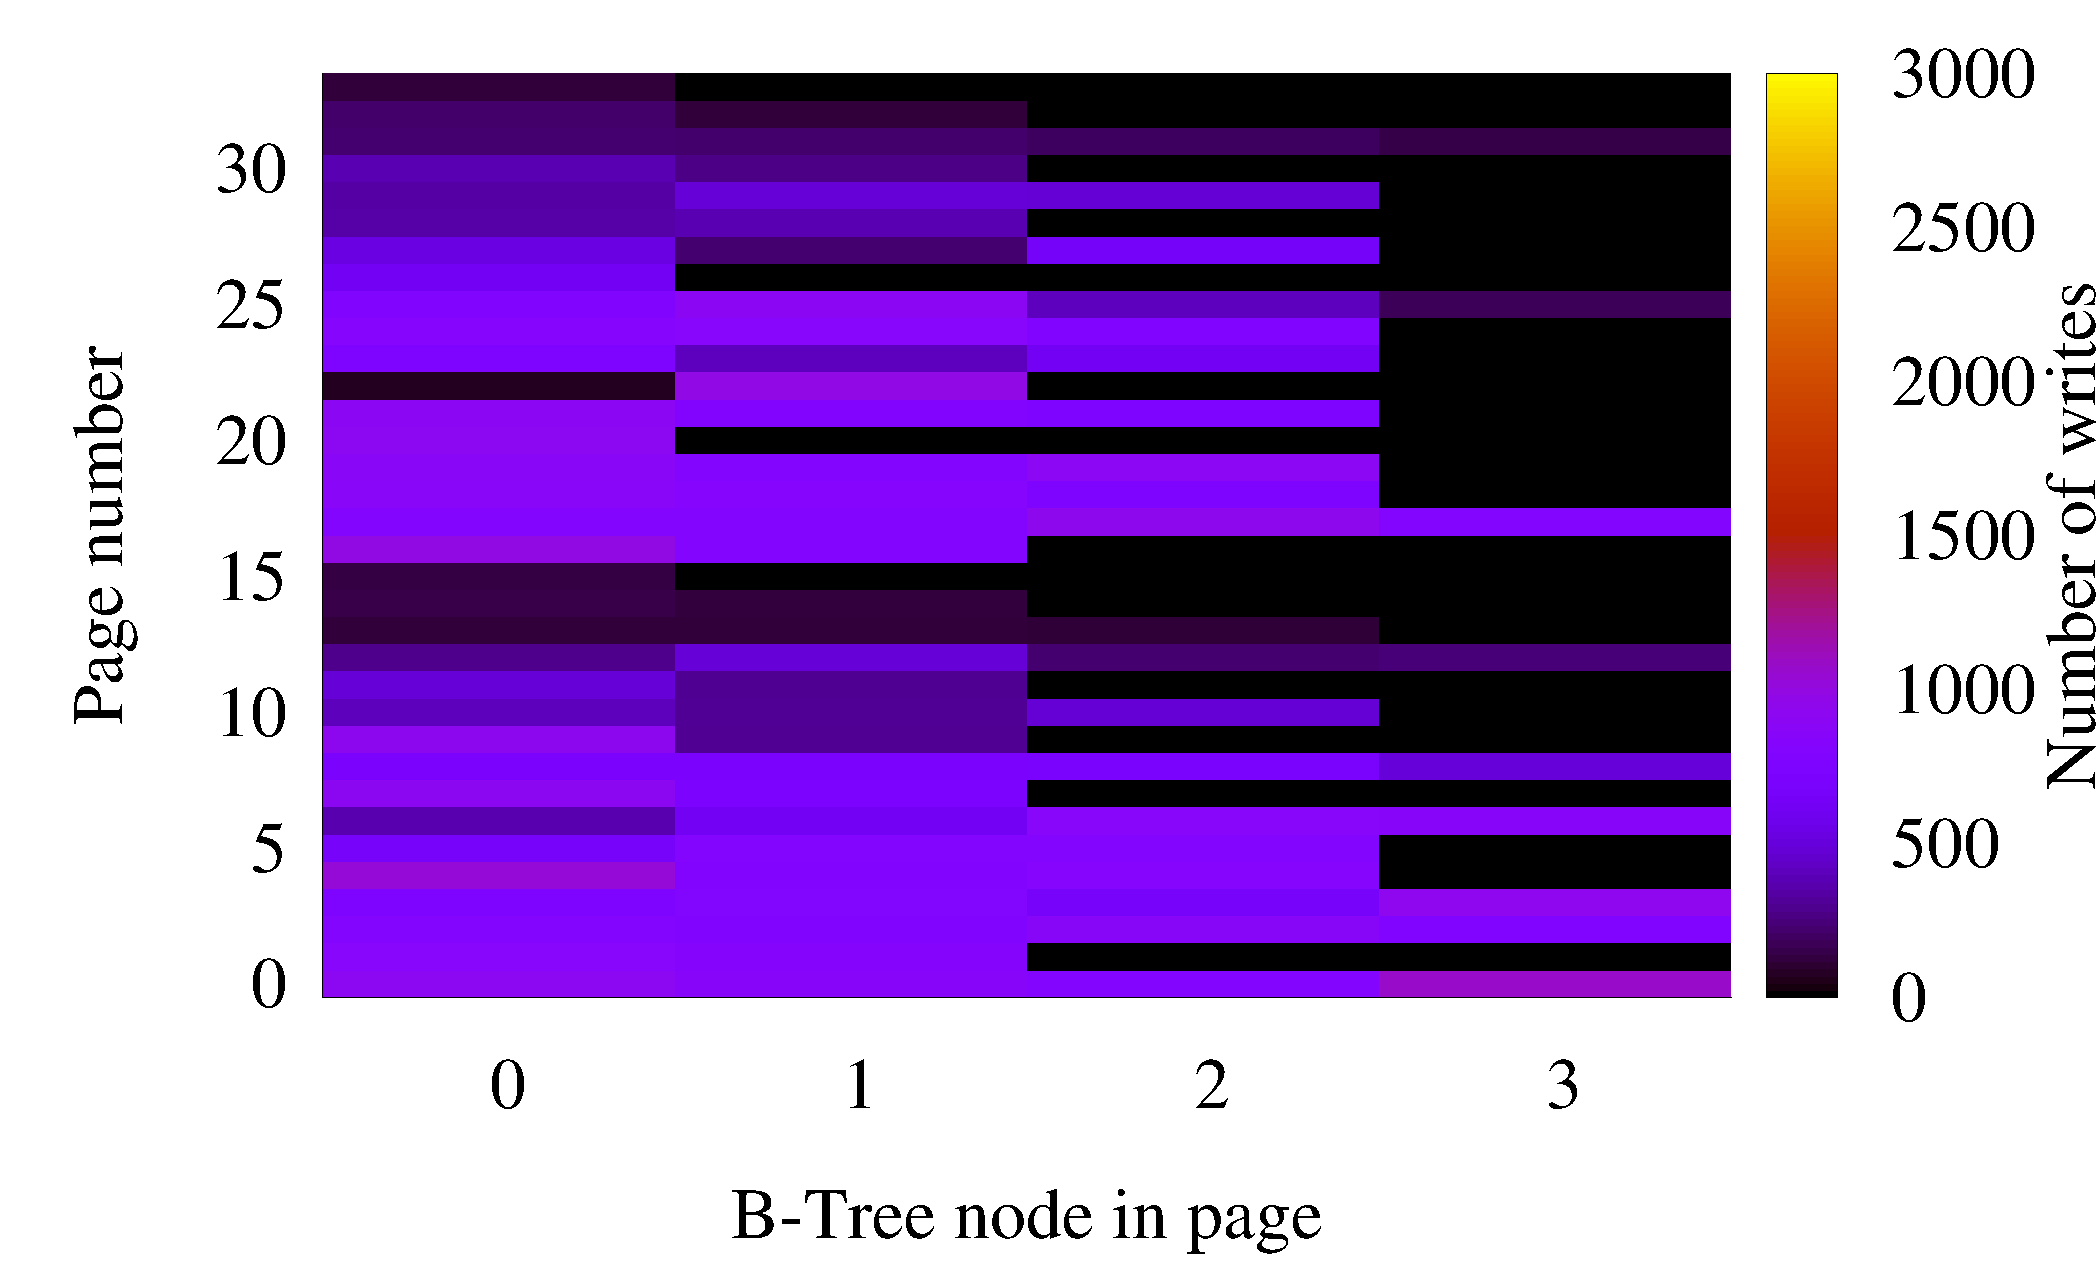
\includegraphics[width=\columnwidth]{figs/write-locations-cdds}
\caption{Heat map of writes in CDDS B-Tree}
\label{fig:write-loc-cdds}
\end{minipage}
\begin{minipage}[b]{0.49\linewidth}
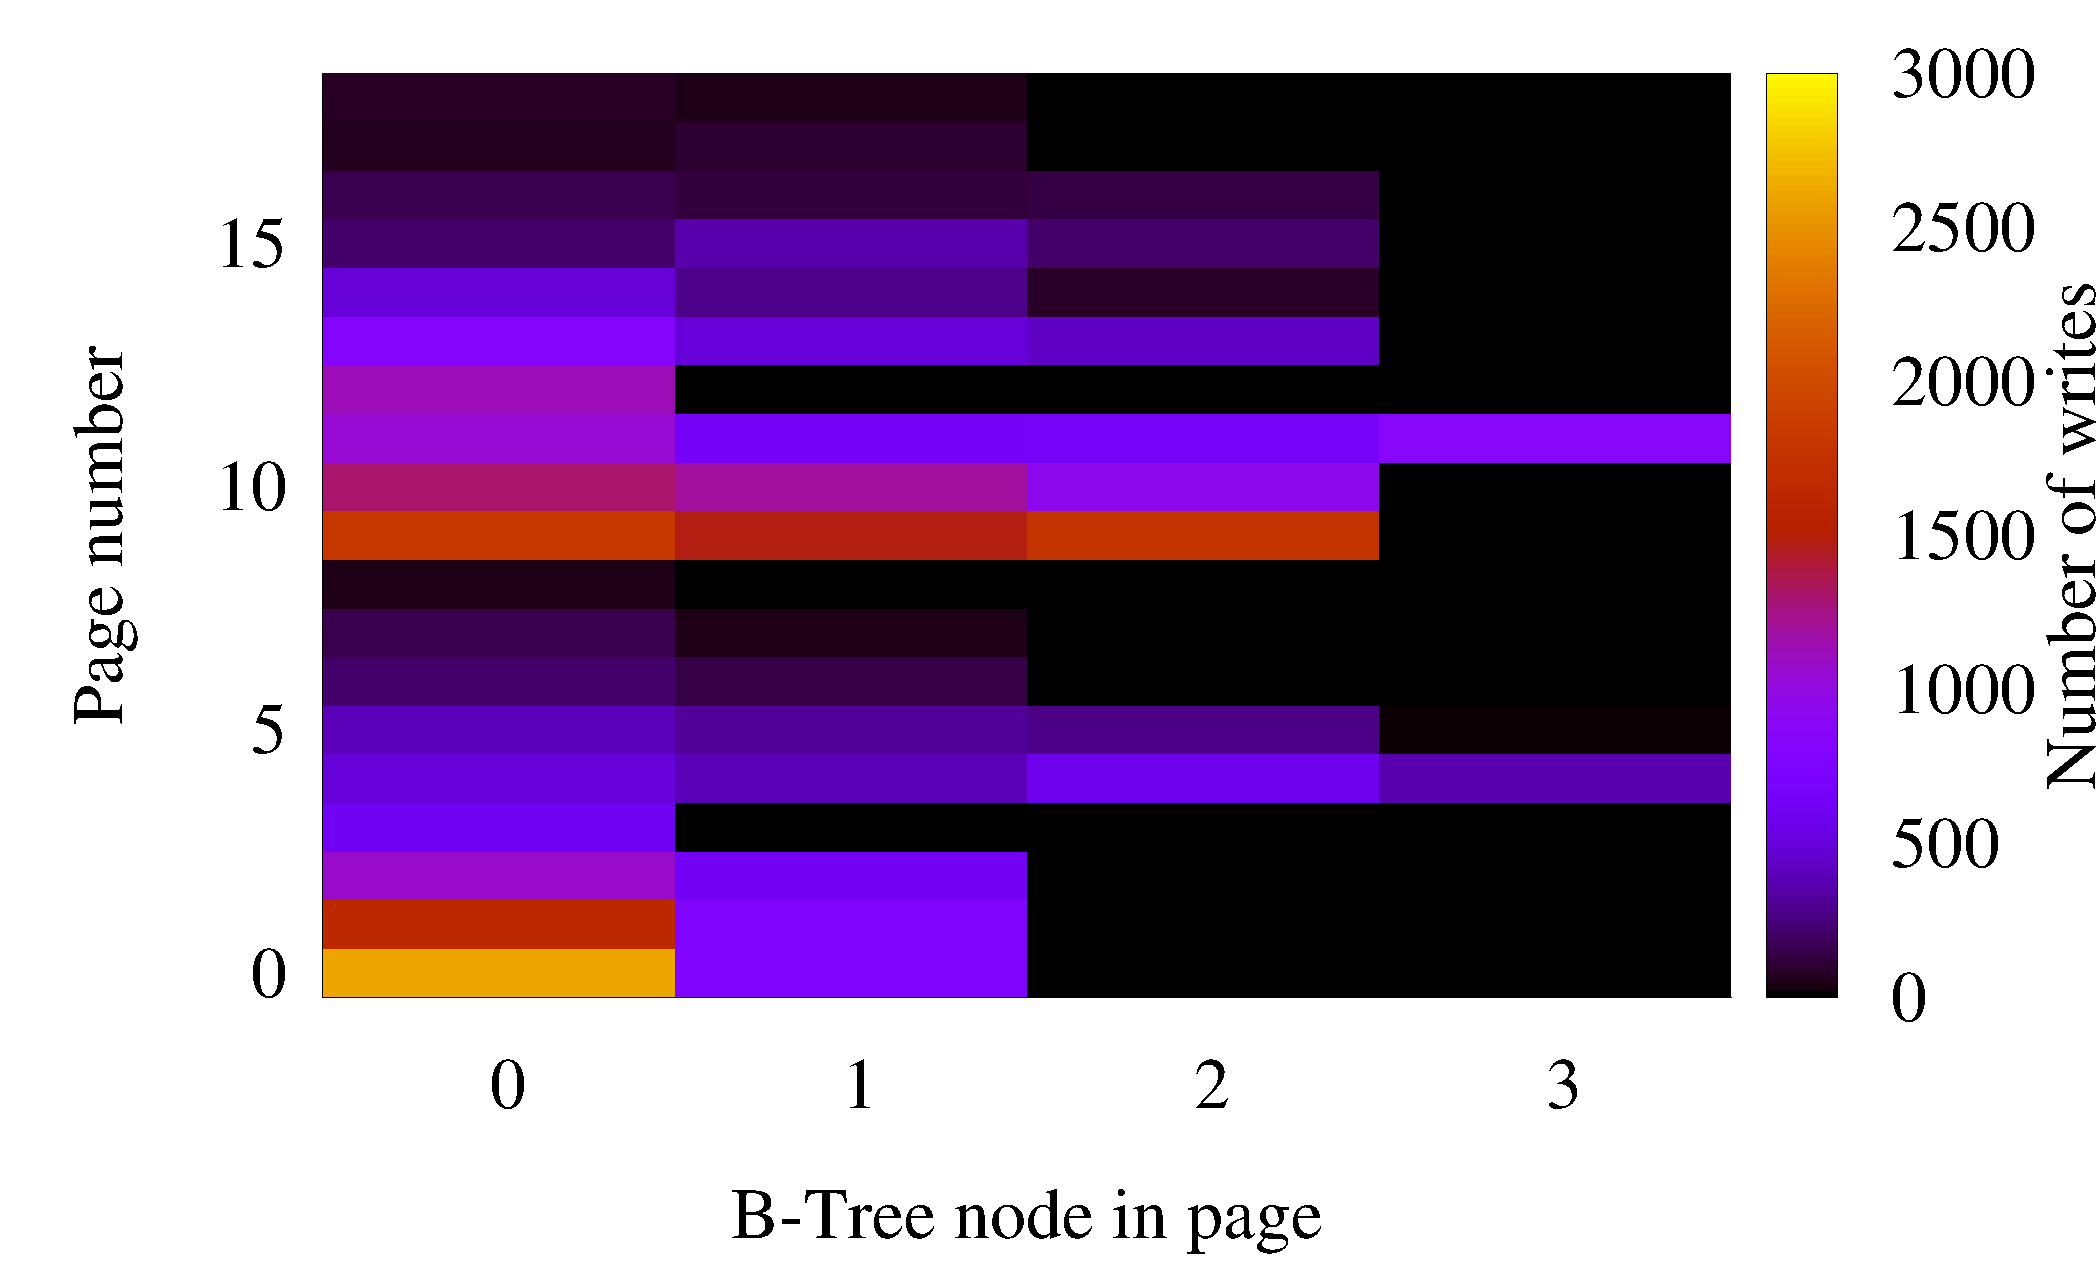
\includegraphics[width=\columnwidth]{figs/write-locations-stx}
\caption{Heat map of writes in STX B-Tree}
\label{fig:write-loc-stx}
\end{minipage}
\end{figure}

\section{Write Frequency by Location}
In order to measure how CDDS-versioning can help in wear-leveling, we profile
the number of writes made to a CDDS B-Tree and the STX B-Tree. We run the same
benchmark used in Section~\ref{sec:api_microbench} but insert only 1000 keys to
help visualize the number of writes per B-Tree node. The keys are chosen
randomly to ensure that they are evenly spread out over the key space and
repeated runs of the experiment produced similar results.  Using the type
information inferred by Cafegrind, we filter the store instructions which are
made on B-Tree nodes during execution. As seen in
Figure~\ref{fig:write-loc-cdds}, Figure~\ref{fig:write-loc-stx} the number of
writes per B-Tree node is distributed in the case of a CDDS B-Tree and there
are no hot spots. The STX B-Tree however has some hot spots which have many
more writes than other locations. It can also be seen that there are 93 B-Tree
nodes created in the CDDS B-Tree while only 47 are used in the STX B-Tree. This
includes leaf nodes and inner nodes created while inserting elements in the
workload.

\begin{figure}[t]
\begin{center}
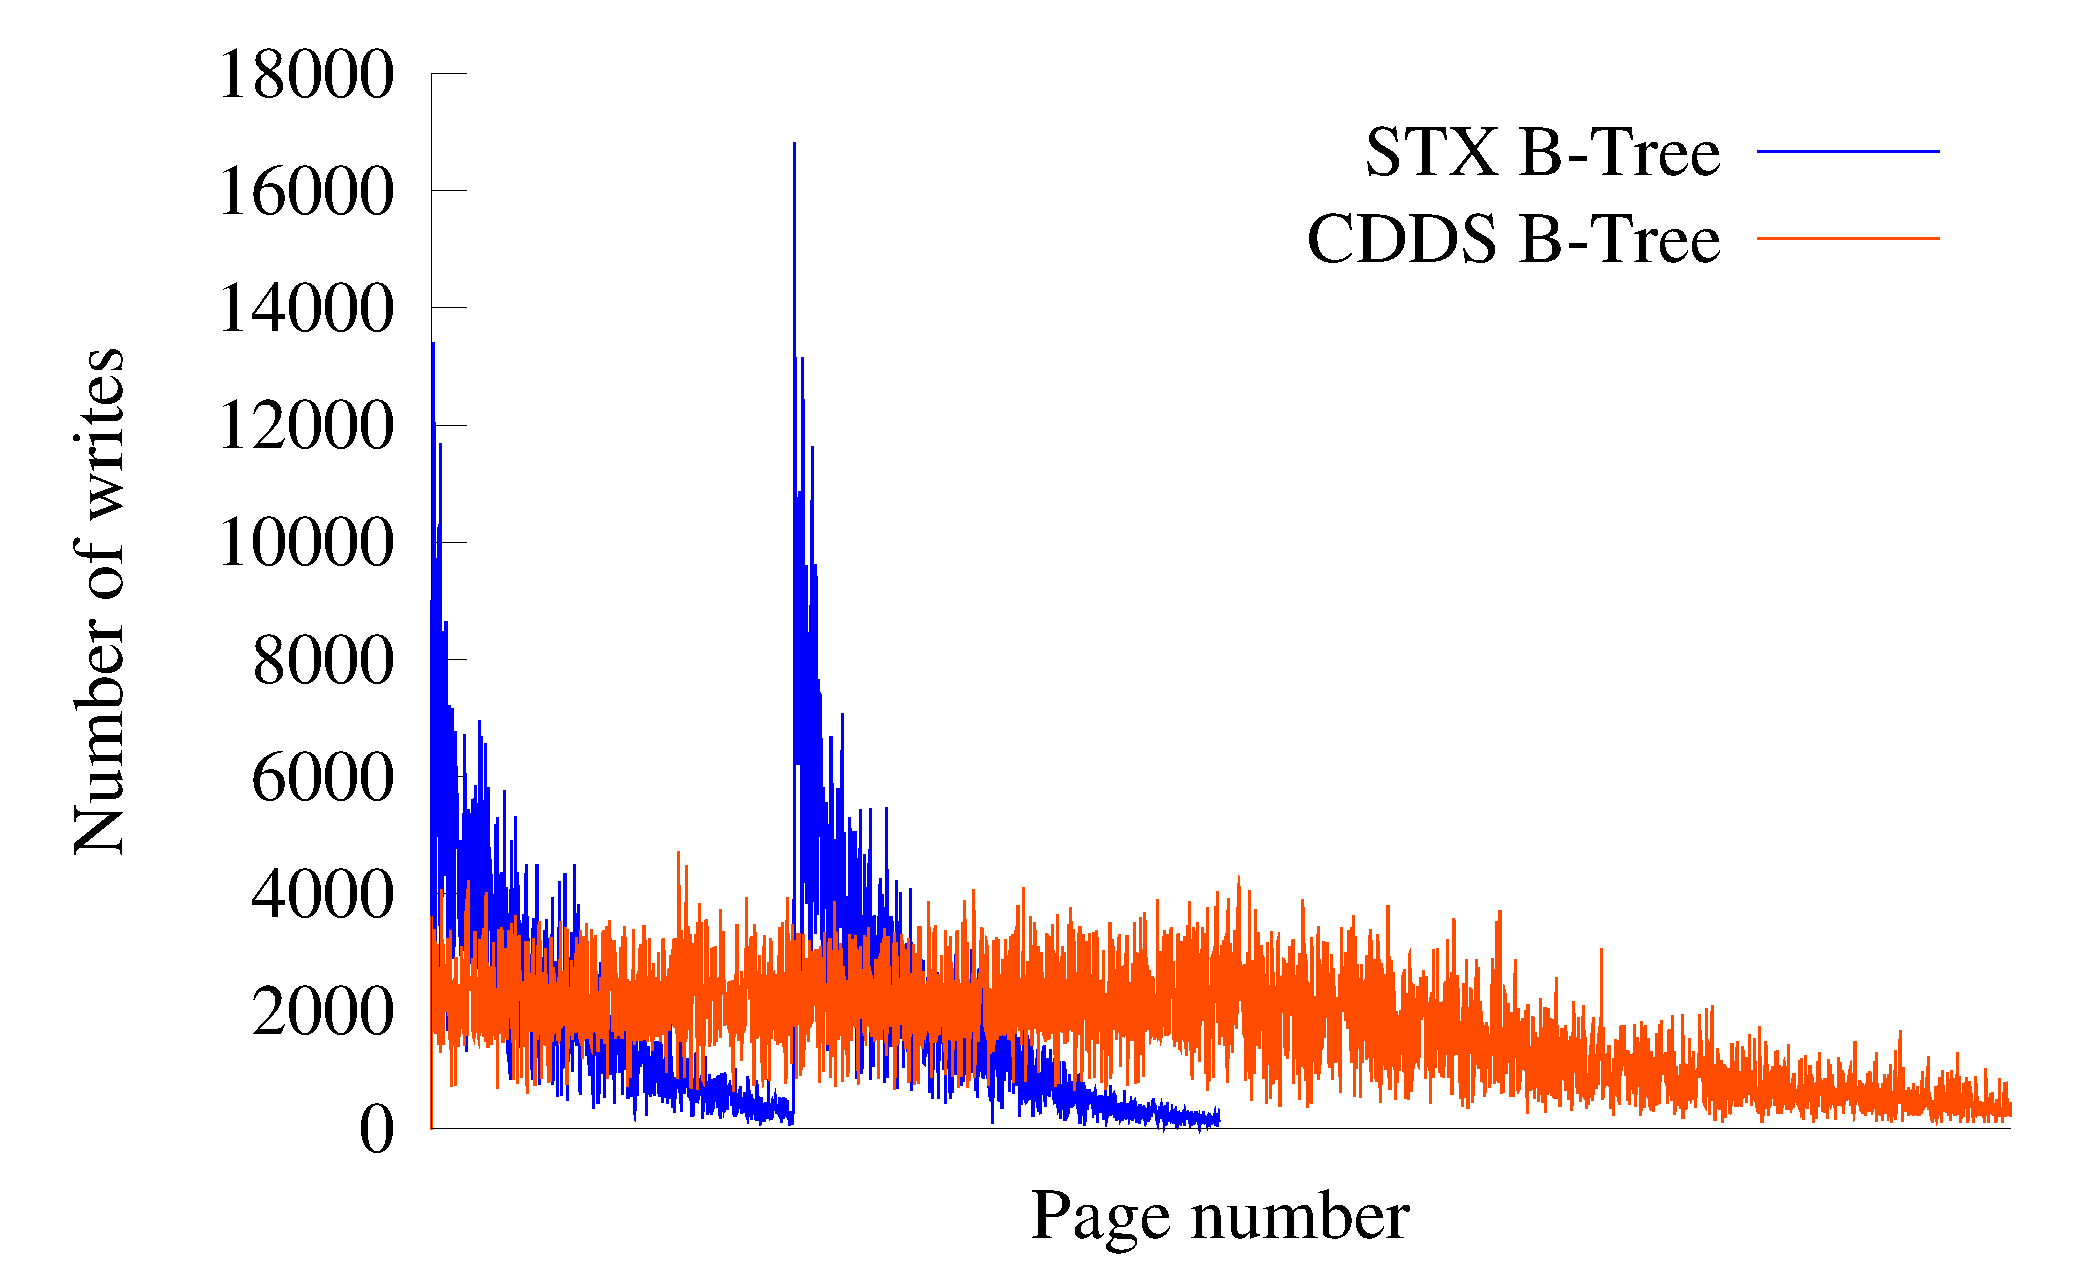
\includegraphics[width=0.7\columnwidth]{figs/wear-line}
\caption{Number of writes per page in CDDS B-Tree and STX B-Tree}
\label{fig:wear-line}
\end{center}
\end{figure}

We repeated the same experiment for a larger number of keys to see how the
number of writes per page varied across a larger number of pages. The results
from an experiment where 100K keys were inserted is shown in
Figure~\ref{fig:wear-line}. In this graph, the number of writes made to a
particular page is plotted for every page used by the application. Similar to
the previous figure, we can see that writes to a CDDS B-Tree are evenly
distributed across a larger number of pages. We can also see that in the
STX B-Tree there are some pages which have up to 16,817 writes, while other pages
have as few as 36 writes during the experiment. Hence we believe that
CDDS-based data structures can be a useful building block to design integrated
wear-leveling solutions for NVBM.
 
\begin{figure}[t]
\begin{center}
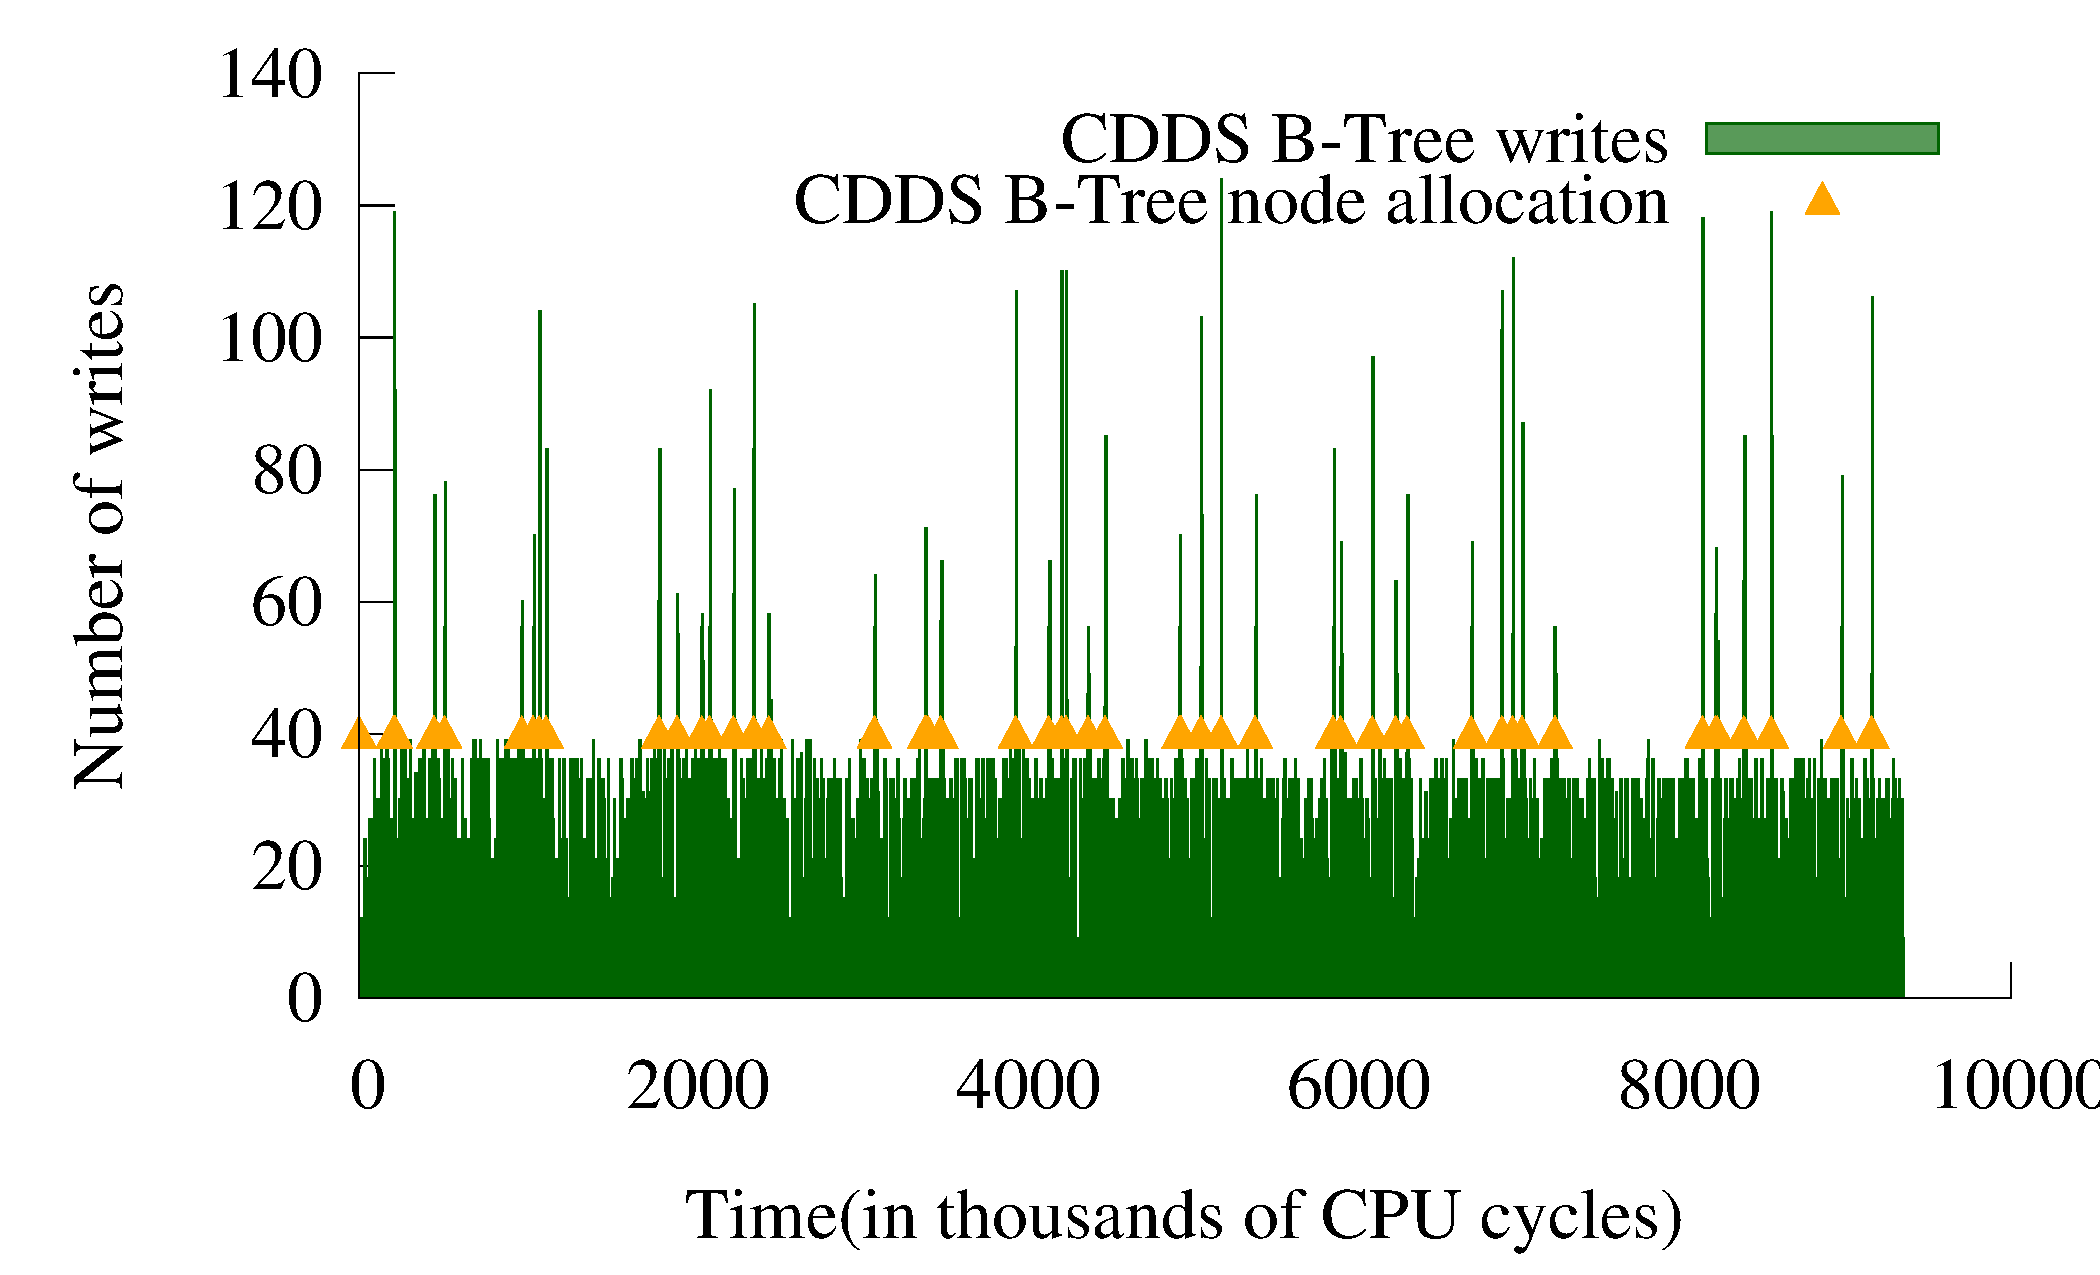
\includegraphics[width=0.7\columnwidth]{figs/write-malloc}
\caption{Writes and Memory allocation events in CDDS B-Tree}
\label{fig:write-time-cdds}
\end{center}
\end{figure}

\section{Write Frequency by Time}
Profiling the CDDS B-Tree using Cafegrind also helps us understand how many
writes are sent to NVBM over time. We can also check if there are some events
which cause a sudden increase in the number of writes. Running the same
micro-benchmark, described in the previous section, we plot the number of
writes that happen with respect to time in CPU clock cycles. In
figure~\ref{fig:write-time-cdds}, writes to B-Tree nodes are categorized into
bins, where a bin corresponds to 2000 CPU cycles. We also plot the allocation
of new B-Tree nodes in the same figure. We can see that when new nodes are
created due to a \texttt{split\_insert}, a large number of writes are made to
NVBM.

\begin{figure}[t]
\begin{center}
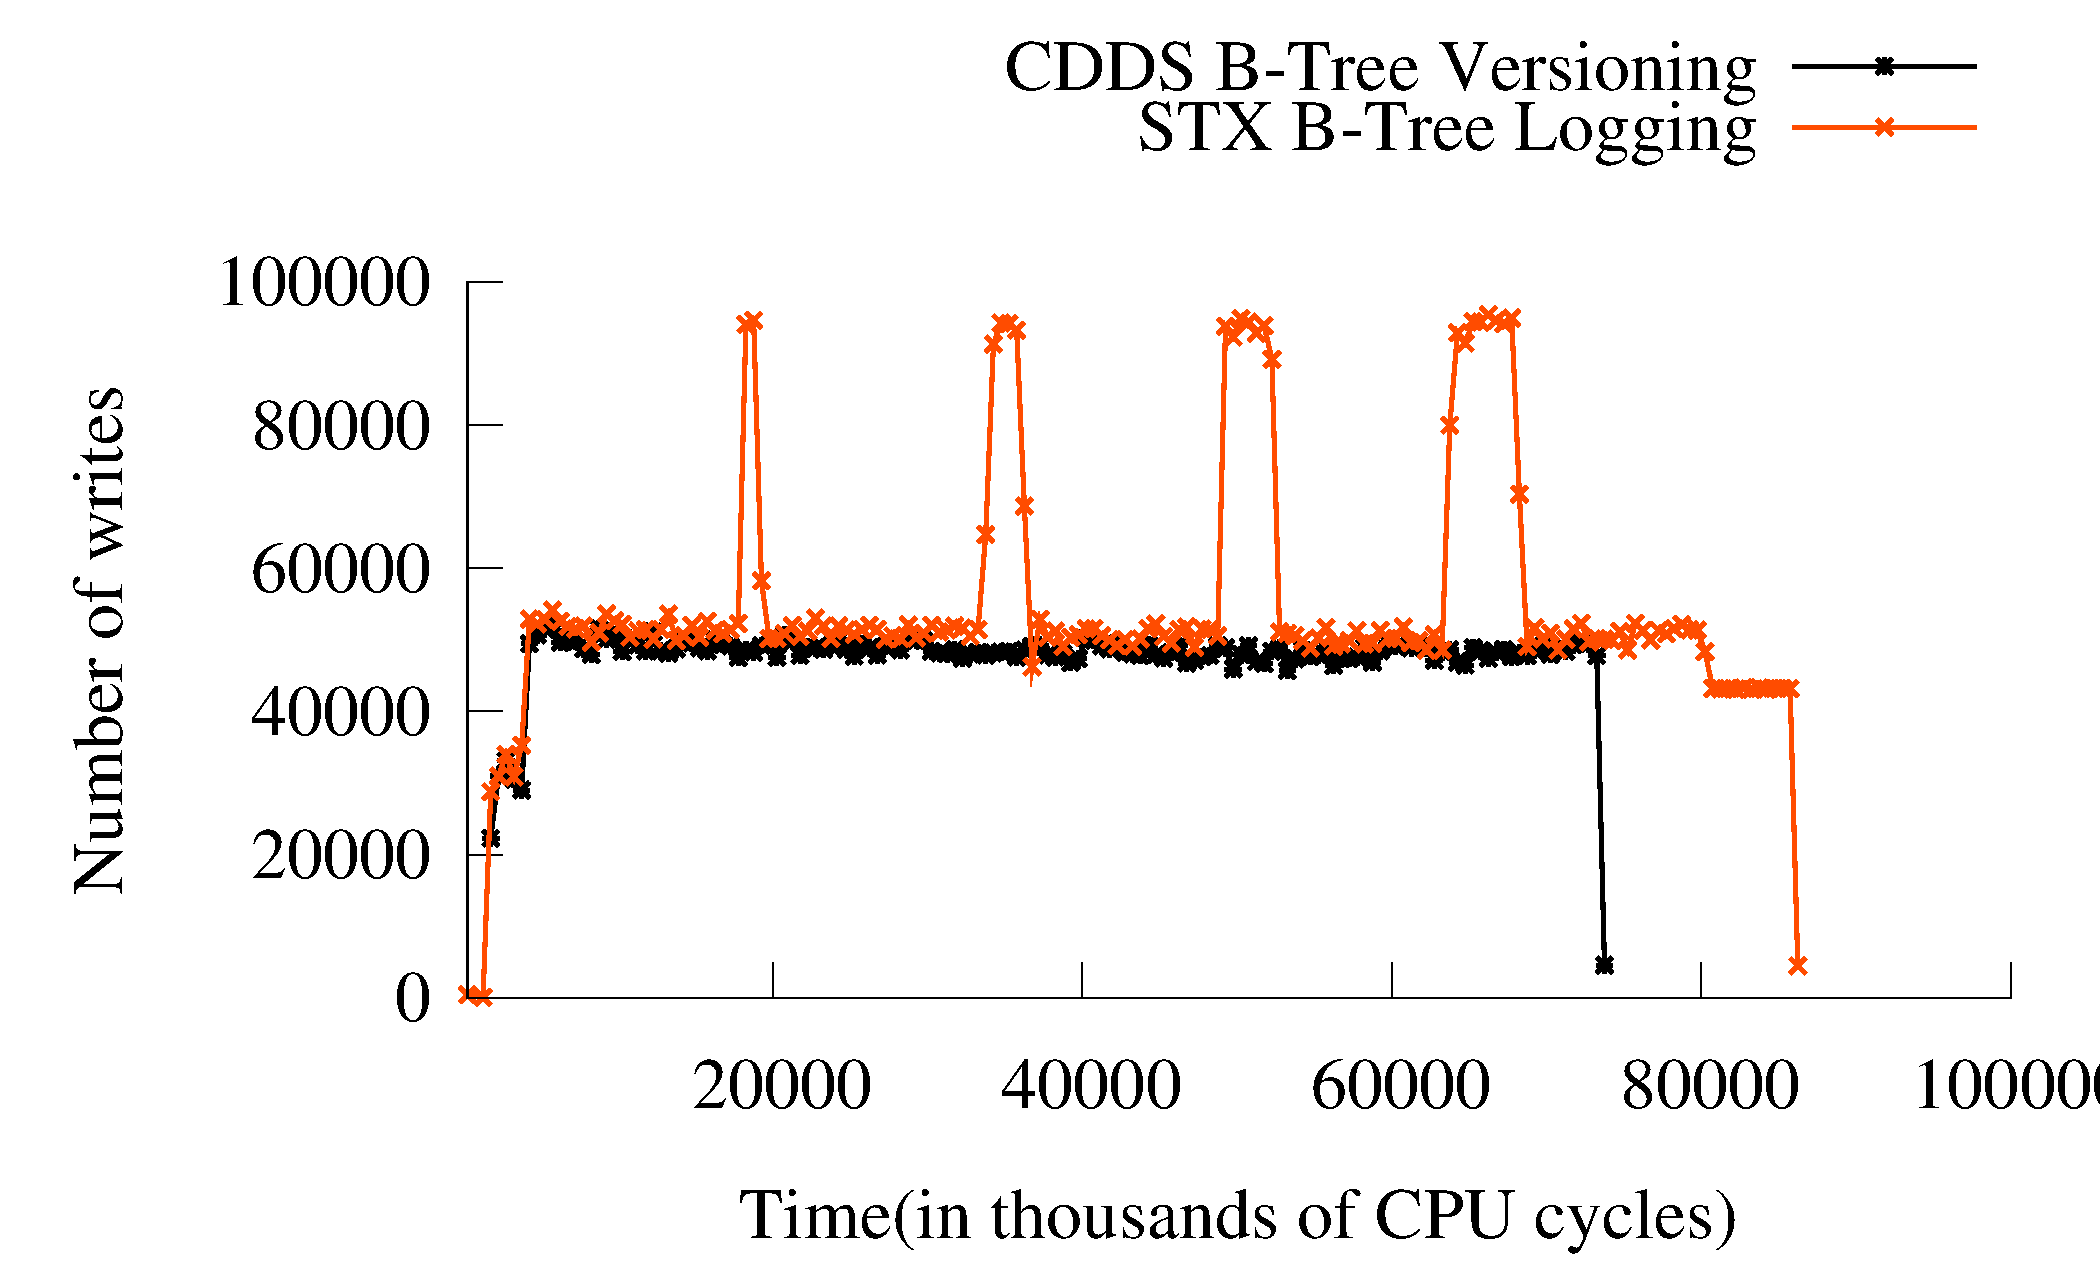
\includegraphics[width=0.7\columnwidth]{figs/write-freq}
\caption{Writes for Versioning vs.\ Logging}
\label{fig:write-freq}
\end{center}
\end{figure}

\section{Profiling Versioning vs.\ Logging}
To compare the performance of the versioning scheme used in Tembo against the
write-ahead logging scheme used in Redis we compared the throughput for both
configurations in Section~\ref{sec:versioning_logging}. Using Cafegrind, we can
gain further insight into the memory operations performed in both cases and
analyze how they affect the throughput. We repeated the experiment performed
in Section~\ref{sec:versioning_logging}, but used 10000 inserts because of the
overhead imposed by profiling. The results, shown in
Figure~\ref{fig:write-freq} show that the versioning scheme used by Tembo has
fewer writes compared to the write-ahead logging scheme. We also found that the
periodic extra writes in the write-ahead logging scheme were due to log
compaction operations. Finally we can see that the CDDS-based experiment
finishes earlier than the logging-based experiment, confirming our earlier
result in which the Tembo had a higher throughput compared to Redis.

\section{Discussion}
Although memory profiling does help us understand the behavior of CDDS, there are
some limitations to this approach. Tracing writes to NVBM locations does not 
take into account the multi-level cache design in a processor. Also, the memory
allocator and wear-leveling algorithms can change the write frequency from an
application to NVBM. However, given that NVBM is not yet commercially available,
we believe that memory profiling is a useful approach to compare different
software designs. Memory profilers can also be used to analyze how software 
systems are affected by asymmetric read/write latencies of NVBM~\cite{Qureshi10}. 

